\section{Experiments}

We have measured the overhead of the PCAST OpenACC autocompare implementation to demonstrate its usability.
We used three of the SPEC ACCEL v1.2 benchmarks, using the \emph{test} dataset.
In each case, the program has an outer time step loop containing the main computation.
The times shown are in seconds, and these are officially SPEC \emph{estimates}, since they were not run in the SPEC harness.
The host machine was a 6-core Intel Haswell (core i7-5820K) with a 3.30GHz clock, with an NVIDIA Tesla Kepler K40c GPU.
We used the default autocompare options, but set a relative tolerance.
The values shown in Table~\ref{res1} and Figure~\ref{fig:sle_figure} are:
\begin{itemize}
\item Time (seconds) to run the test data set sequentially on the CPU.
\item Time (seconds) to run the test data set in parallel on the GPU.
\item Time (seconds) to run the test data set redundantly on both CPU and GPU without the autocompare feature enabled.
\item Time (seconds) to run the test data set redundantly on both CPU and GPU using the autocompare feature.
\item Number of variables or arrays compared.
\item Number of data values compared.
\end{itemize}


\begin{figure*}[t]
    \centering
    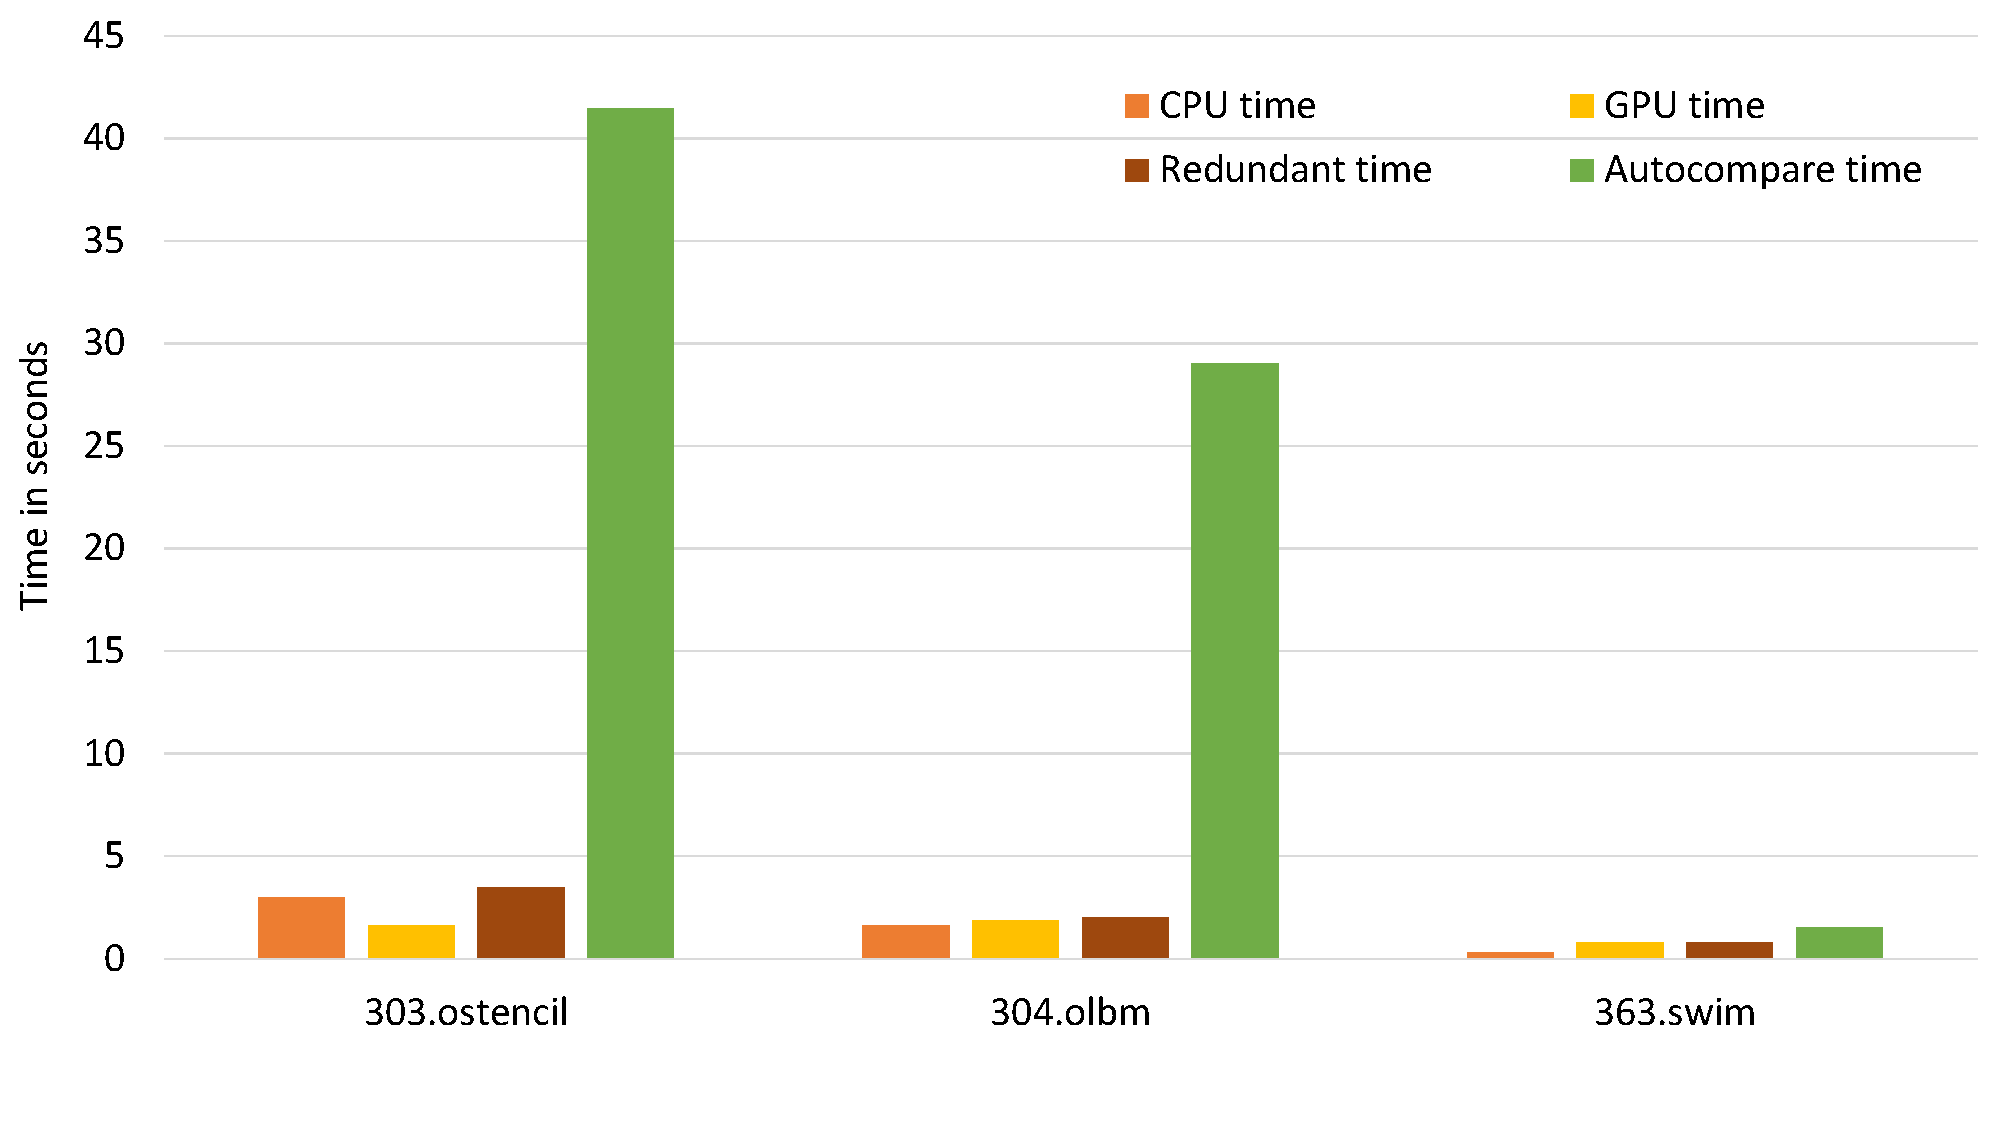
\includegraphics [width=1\linewidth] {Table1.pdf}
    \caption{Results showing overhead of OpenACC autocompare.}
    \label{fig:sle_figure}
\end{figure*}


\begin{table}
\begin{center}
\begin{tabular}{rrrl}
\hline
303.ostencil & 304.olbm & 363.swim & \\
\hline
 3.01s &  1.61s & 0.33s & CPU time (sequential) \\
 1.61s &  1.85s & 0.78s & GPU time \\
 3.48s &  2.00s & 0.81s & redundant execution on CPU and GPU \\
41.46s & 29.05s & 1.53s & autocompare time \\
202 & 61 & 258 & variables and arrays compared \\
3,388,997,632 & 1,586,800,000 & 67,897,602 & values compared \\
\hline
\end{tabular}
\end{center}
\caption{Results showing overhead of OpenACC autocompare.}
\label{res1}
\end{table}

The two costs of the autocompare feature are running the compute region on both CPU and GPU, and downloading and comparing the values.
The cost of redundant execution is less than the sum of the CPU and GPU times, because the GPU code executes asynchronously while the CPU executes the corresponding code.
Since this is a feature used during code development and debugging, we consider this to be relatively low overhead.
The cost of doing the many floating point comparisons is significant, and seems directly related to the number of data items compared, and unrelated to the number of arrays or variables being compared.
However, using this feature to find where a GPU computation diverges moves the cost from the programmer to the computer, so it could be invaluable regardless of the overhead.

One side note: the \emph{test} datasets used here are relatively small.
Even so, we had to set the relative tolerance to avoid the comparisons detecting differences due to different summation accumulation order.
In fact, there were so many tolerated floating-point differences, that we do not consider the idea to compute and compare checksums first, since the checksums would most often be different even though the actual differences would then be tolerated.
